%----------------------------------------------------------------------------------------
%	PACKAGES AND OTHER DOCUMENT CONFIGURATIONS
%----------------------------------------------------------------------------------------

\documentclass[a0paper,portrait]{baposter}

\usepackage[font=small,labelfont=bf]{caption} % Required for specifying captions to tables and figures
\usepackage{booktabs} % Horizontal rules in tables
\usepackage{relsize} % Used for making text smaller in some places

\usepackage{amsmath,amsfonts,amssymb,amsthm} % Math packages
\usepackage{eqparbox}

\usepackage{textcomp}

\usepackage[brazil]{babel}
\usepackage[utf8]{inputenc}


\graphicspath{{figures/}} % Directory in which figures are stored

 \definecolor{bordercol}{RGB}{45, 235, 118} % Border color of content boxes
 \definecolor{headercol1}{RGB}{5, 184, 255} % Background color for the header in the content boxes (left side)
 \definecolor{headercol2}{RGB}{26, 167, 85} % Background color for the header in the content boxes (right side)
 \definecolor{headerfontcol}{RGB}{0, 0, 0} % Text color for the header text in the content boxes
 \definecolor{boxcolor}{RGB}{255, 255, 255} % Background color for the content in the content boxes


\begin{document}

\background{% Set the background to an image (background.pdf)
\begin{tikzpicture}[remember picture,overlay]
\draw (current page.north west)+(-2em,2em) node[anchor=north west]
{
\includegraphics[height=1.1\textheight]{background}};
\end{tikzpicture}
}

\begin{poster}
{grid=false,
borderColor=bordercol, % Border color of content boxes
headerColorOne=headercol1, % Background color for the header in the content boxes (left side)
headerColorTwo=headercol2, % Background color for the header in the content boxes (right side)
headerFontColor=headerfontcol, % Text color for the header text in the content boxes
boxColorOne=boxcolor, % Background color for the content in the content boxes
headershape=roundedright, % Specify the rounded corner in the content box headers
headerfont=\Large\sf\bf, % Font modifiers for the text in the content box headers
textborder=rectangle,
background=user,
headerborder=open, % Change to closed for a line under the content box headers
boxshade=plain
}
{\begin{tabular}{c}
        
\includegraphics[height=1cm]{UNIVAP-SF.png}\\
\end{tabular}
}  
%
%----------------------------------------------------------------------------------------
%	TITLE AND AUTHOR NAME
%----------------------------------------------------------------------------------------
%
{\bf  \LARGE {DECIMETRIC RADIO EMISSION ANALYSIS OF CHROMOSPHERIC EVAPORATION IN A X1.0 FLARE ON MARCH 29, 2014} \\ % Poster title
\vspace{0.2cm} 
\footnotesize \underline{André Rossi Korol}, Francisco Carlos Rocha Fernandes\\  % Author names
\footnotesize \it UNIVAP --- Universidade do Vale do Paraíba\\ % Institution names
\footnotesize \it \textcolor{blue}{\underline{anrobits@yahoo.com.br}}\/}
%Author email addresses

{\begin{tabular}{c}
        
\includegraphics[height=1cm]{ipd2-sf.png}
\end{tabular}
}  

%----------------------------------------------------------------------------------------
%	RESUMO
%----------------------------------------------------------------------------------------
\headerbox{Abstract}{name=abstract,span=1,column=0,row=0}
{O pôster deve ser elaborado para papel a0, em duas ou três colunas, devendo conter, obrigatoriamente o título, o nome dos autores com a sigla das suas respectivas instituições e o email do primeiro autor. 
Será obrigatória a presença do autor apresentador durante a apresentação do pôster.


\textit{Keywords: solar flare, solar radio emission,}\newline
\textit{chromospheric evaporation, spectrometer,}\newline
\textit{data analysis, data visualization.}
%Cabe aos autores providenciarem o pôster em material adequado (lona, pvc, glosspaper ou similar) com corda para ser afixado.
}

%---------------------------------------------------------------------------------------
%   INTRODUÇÃO
%---------------------------------------------------------------------------------------

\headerbox{Introduction}{name=introduction,span=1,column=0,below=abstract}
{Algumas dicas:
O pôster deverá ter informações referentes à sua pesquisa, informações tais como: Resumo, Introdução, Objetivo, Metodologia, Conclusão e outras informações (estes são pontos de orientação geral e não são regras).
Utilize tamanho de fonte 48 como mínimo para título e fonte 28 como mínimo para conteúdo.
Figuras e tabelas deverão cobrir, no máximo, $50\%$ do pôster, informando a fonte dos dados contidos nas mesmas. A fonte deverá ser colocada abaixo das figuras e tabelas.
As informações apresentadas no pôster devem ser concisas e claras.
Este modelo já se encontra na formatação sugerida.}


%----------------------------------------------------------------------------------------
%	OBJETIVOS
%----------------------------------------------------------------------------------------



\headerbox{Objectives}{name=objectives,span=1,column=0,below=introduction}
{Nessa seção deve-se apresentar um parágrafo descrevendo o objetivo geral e alguns itens indicando os objetivos específicos. Pode-se utilizar o ambiente \texttt{itemize} como abaixo.

\begin{itemize}
    \item Objetivo específico 1
    \item Objetivo específico 2
    \item Objetivo específico 3
\end{itemize}

\vspace{9cm}

}

%----------------------------------------------------------------------------------------
%	METODOLOGIA 
%----------------------------------------------------------------------------------------
\headerbox{Methodology}{name=methodology,span=1,column=1,row=0}
{Pode-se incluir tabelas utilizando o ambiente \texttt{table} ou conforme apresentado abaixo.

Enquanto equações são organizadas utilizando o ambiente \texttt{equation}, como segue:
}

%----------------------------------------------------------------------------------------
%	RESULTADO
%----------------------------------------------------------------------------------------
\headerbox{Results and Discussions}{name=results,span=1,column=1,below=methodology}
{Pode-se incluir figuras utilizando o ambiente \texttt{includegraphics} ou conforme apresentado abaixo.

\begin{center}
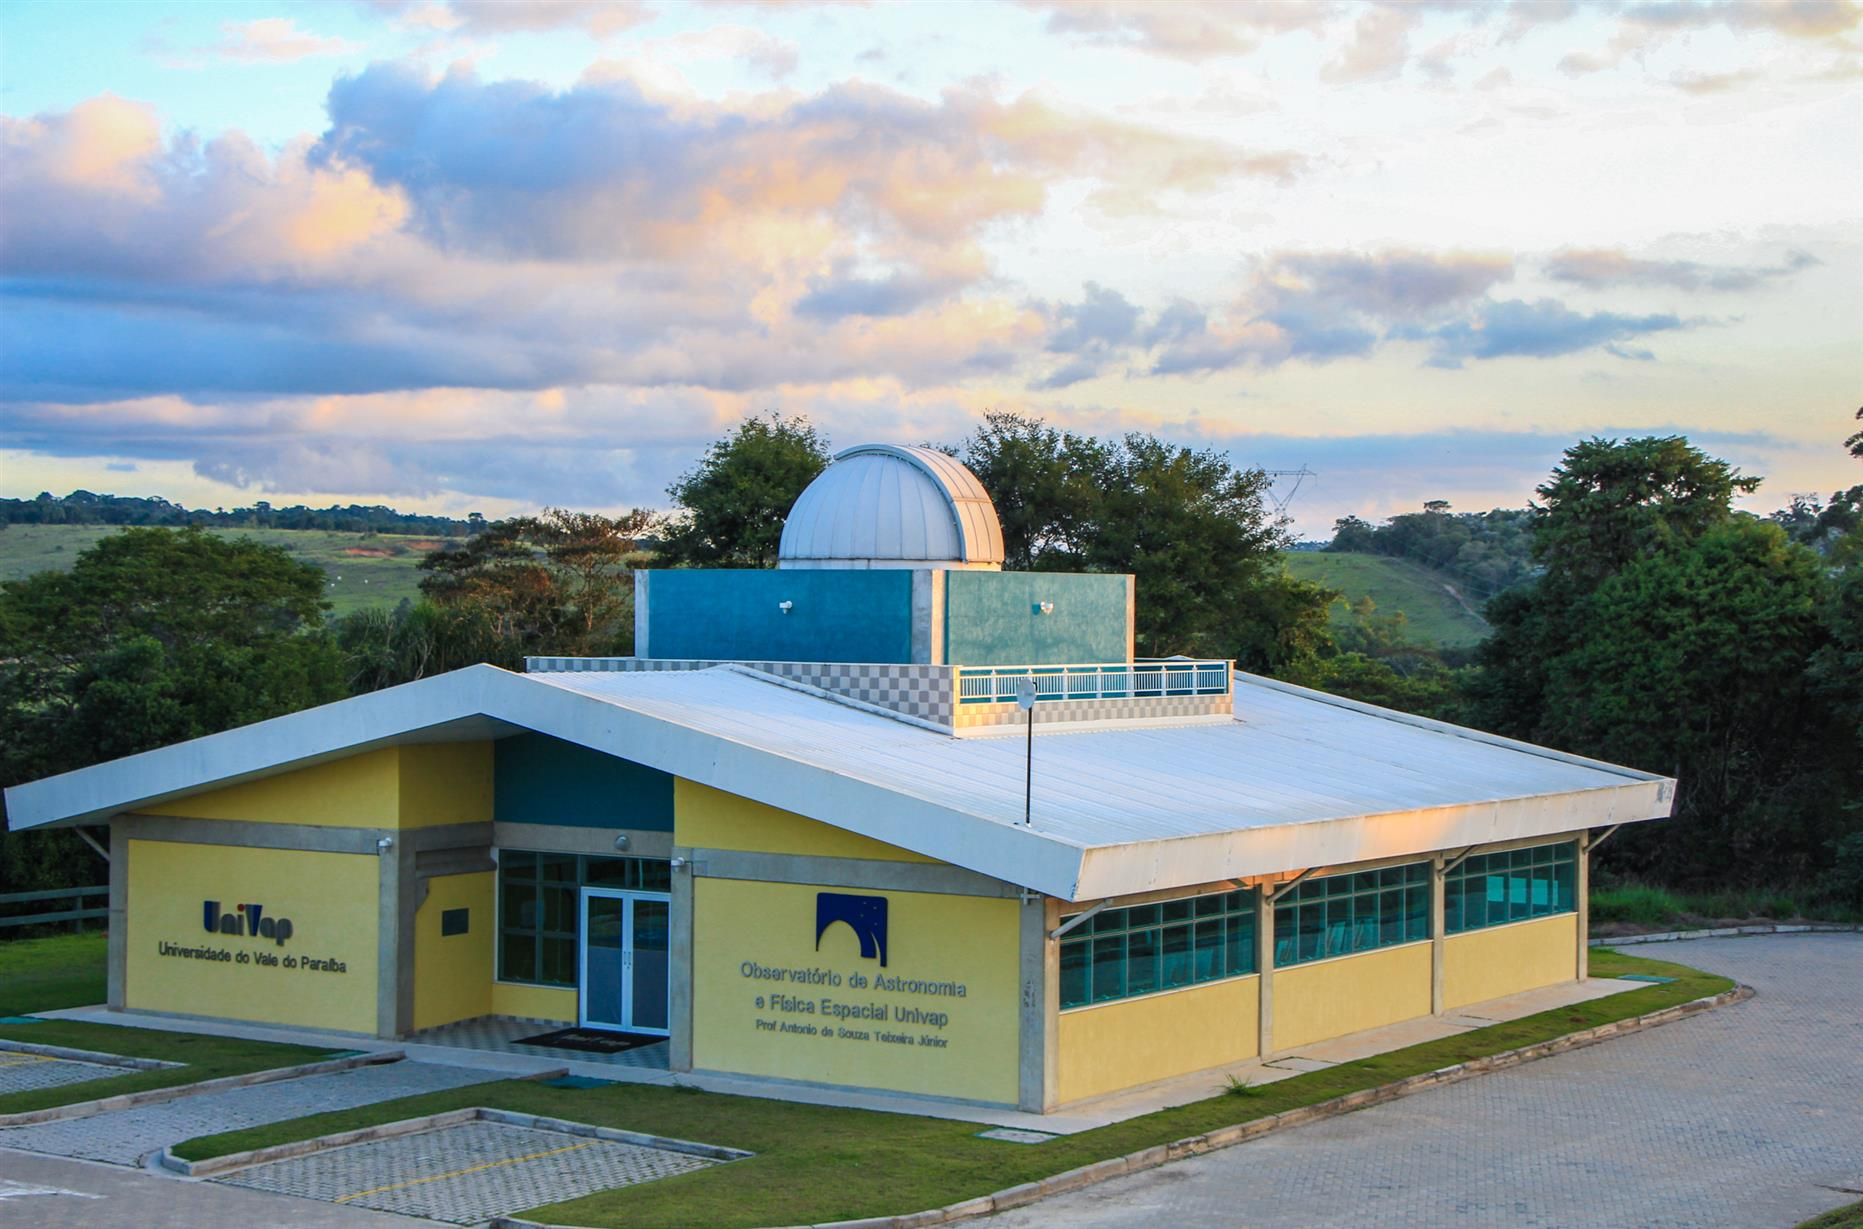
\includegraphics[width=0.8\textwidth]{figures/observatorio.jpg}\\
Figura 1. Posicionar legenda abaixo da imagem, espaçamento simples.\\
Fonte: do autor.
\end{center}

\vspace{1.3cm}
\vspace{9cm}

}

%----------------------------------------------------------------------------------------
%	DISCUSSÃO
%----------------------------------------------------------------------------------------
\headerbox{Conclusions}{name=conclusions,column=2,row=0} % To reduce this block to 1 column width, remove 'span=2'
{Sugestões para fazer uma conclusão:
\begin{itemize}
    \item Fazer um breve resumo do trabalho.
    \item Referir qual foi a grande conclusão do trabalho.
    \item Referir se concretizaram ou não todos os objetivos ou se não foi possível concretizar algum deles e explicar o porquê.
    \item Referir a importância que o trabalho tem para sua pesquisa. 
\end{itemize}

\vspace{1.5cm}

}

%----------------------------------------------------------------------------------------
%	AGRADECIMENTOS
%----------------------------------------------------------------------------------------
\headerbox{Acknowledgements}{name=acknowledgements,column=2,below=conclusions,span=1}
{Agradecimentos a instituições de fomento ou a colaboradores do projeto.
}

%----------------------------------------------------------------------------------------
%	REFERENCIAS
%----------------------------------------------------------------------------------------
\headerbox{References}{name=references,column=2,below=acknowledgements,span=1}
{Listar as referências listadas no texto. Exemplo de citações:\\

[1] L. Burlaga, \textit{et.al} Magnetic loop behind an interplanetary shock; Voyager, helios, and imp 8 observations. {\it J. Geoph. Res.: Space Physics}, Wiley Online Library, v. 86, n. A8, p. 6673--6684, 1981.

[2] T. Wolfgang, \textit{Introduction: The Ellipsoidal Earth Model.} In: WOLFGANG, Torge. \textit{Geodesy.} 3.\ ed. New York: De Gruyter, 2001.\ cap. 1, p. 8.

[3] D. S. Wilks, \textit{Statistical methods in the atmospheric sciences}. Acad. Press San Diego, 1995.

\vspace{9cm}
}

%----------------------------------------------------------------------------------------
%	REALIZAÇÃO
%----------------------------------------------------------------------------------------

\headerbox{Realization}{name=event,column=0,below=references, above=bottom,span=3}
{\begin{center}
    
\includegraphics[width=0.7\textwidth]{rodape_simfast.png}
\end{center}
} 


\end{poster}

\end{document}
